\documentclass{beamer}
\mode<presentation>
\usetheme{CambridgeUS}
\usepackage[russian]{babel}
\usepackage[utf8]{inputenc}
\usepackage[T2A]{fontenc}
\usepackage{sansmathaccent}

\usepackage{verbatim}
\usepackage{alltt}

\pdfmapfile{+sansmathaccent.map}
\title[Массивы]{Множественный тип данных}
\author{Наумов Д.А., доц. каф. КТ, ИТГД }
\date[12.12.2019] {Алгоритмические языки и программирование, 2019}

\begin{document}

%ТИТУЛЬНЫЙ СЛАЙД
\begin{frame}
  \titlepage
\end{frame}
  
%СОДЕРЖАНИЕ ЛЕКЦИИ
\begin{frame}
  \frametitle{Содержание лекции}
  \tableofcontents  
\end{frame}
  
%РАЗДЕЛ 1
\section{Элементы теории множеств}
\subsection{Понятия и определения}
\begin{frame}
Множество — одно из ключевых понятий математики; это математический объект, сам являющийся набором, совокупностью, собранием каких-либо объектов, которые называются элементами этого множества и обладают общим для всех их характеристическим свойством.
\begin{block}{Множество может быть}
\begin{itemize}
\item пустым и не пустым;
\item упорядоченным и не упорядоченным;
\item конечным и бесконечным;
\item бесконечное множество - счетным и несчетным;
\end{itemize}
\end{block}
\begin{block}{Элементы множества}
объекты, из которых состоит множество.
\end{block}
\end{frame} 

\begin{frame}
\begin{block}{Принадлежность элемента \textit{a} множеству \textit{A}}
\[a \in A\].
\end{block}
\begin{block}{Не принадлежность элемента \textit{a} множеству \textit{A}}
\[a \notin A\].
\end{block}
\begin{block}{Равенство двух множеств \textit{A = B}}
\[x \in A \Longleftrightarrow x \in B\].
\end{block}
\begin{block}{Способы задания множеств}
\begin{itemize}
\item перечисление $Y = \{0, 2, 4, 8\}$;
\item описание $ Y = \{x \in X | A(x)\} $;
\end{itemize}
\end{block}
\end{frame} 

\subsection{Отношения между множествами}
\begin{frame}
\begin{block}{\textit{A} включено в \textit{B}, если каждый элемент \textit{A} принадлежит \textit{B}}
\[A \subseteq B \Leftrightarrow \forall a\in A: a\in B\].
\end{block}
\begin{block}{\textit{A} включает \textit{B}, если \textit{B} включено в \textit{A}}
\[A \supseteq B \Leftrightarrow B \subseteq A \].
\end{block}
\begin{block}{\textit{A} равно \textit{B}, если \textit{A} и \textit{B} включены друг в друга}
\[A=B \Leftrightarrow (A\subseteq B)\wedge(B\subseteq A) \].
\end{block}
\begin{itemize}
\item $A = A$;
\item если $A = B$, то $B = A$;
\item если $A = B$, $A = B$, то $A = C$;
\end{itemize}
\end{frame}

\begin{frame}
\begin{block}{\textit{A} строго включено в \textit{B}, если \textit{A} включено в \textit{B} и не равное ему}
\[A \subset B \Leftrightarrow (A \subseteq B)\wedge (A \neq B)\].
\end{block}
\begin{block}{\textit{A} строго включает \textit{B}, если \textit{B} строго включено в \textit{A}}
\[A \supset B \Leftrightarrow B \subset A \].
\end{block}
\begin{block}{\textit{A} и \textit{B} не пересекаются, если у них нет общих элементов}
\[A и B не пересекаются \Leftrightarrow \forall a \in A: a \notin B \].
\end{block}
\begin{block}{\textit{A} и \textit{B} находятся в общем положении}
\[ \exists a,b,c: (a\in A)\wedge(a \notin B)\wedge(b\in B)\wedge(b \notin A)\wedge(c\in B)\wedge(c \in B)\].
\end{block}
\end{frame}

\begin{frame}
Диаграмма Венна (также используется название диаграмма Эйлера — Венна) — схематичное изображение всех возможных отношений (объединение, пересечение, разность, симметрическая разность) нескольких (часто — трёх) подмножеств универсального множества.
\begin{figure}[h]
\centering
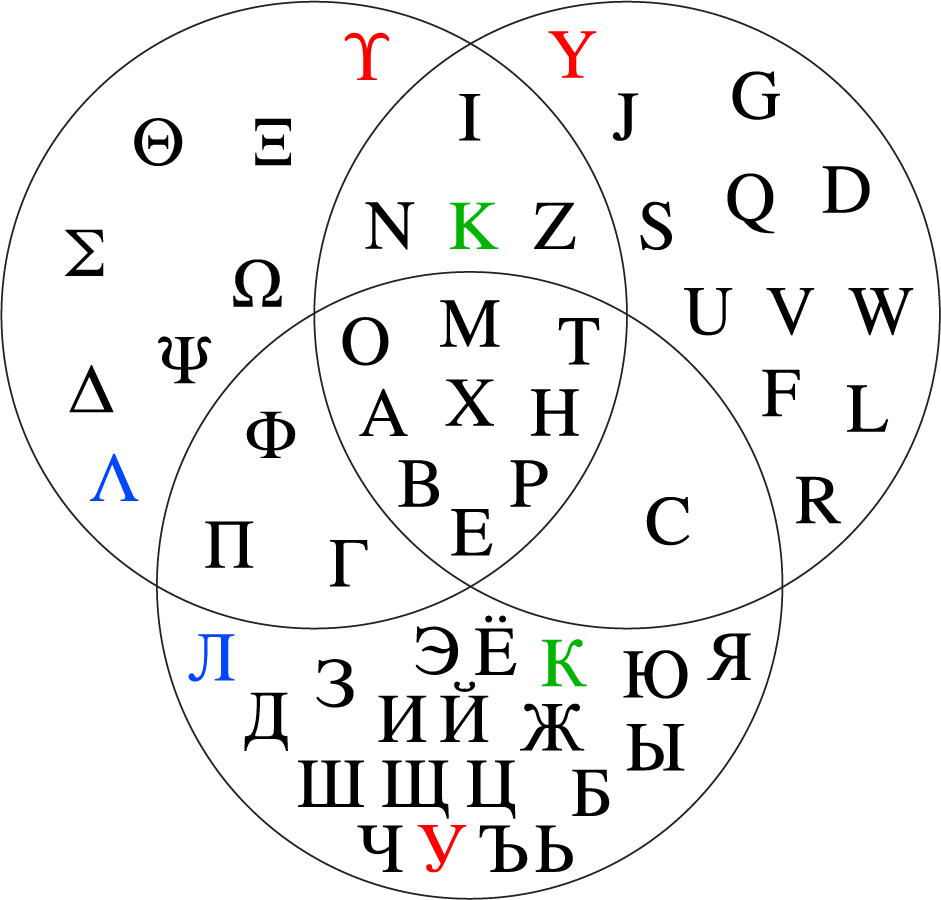
\includegraphics[scale=0.2]{images/venn_diagram.png}
\caption{Диаграмма Венна, показывающая все пересечения графем заглавных букв греческого, русского и латинского алфавитов}
\label{pic-venn}
\end{figure}
Автор: Watchduck (a.k.a. Tilman Piesk) - File:Venn diagram gr la ru.svg, Общественное достояние, https://commons.wikimedia.org/w/index.php?curid=27169804
\end{frame}

\subsection{Операции над множествами}
\begin{frame}{Бинарные операции}
\begin{block}{Пересечение}
\[A\cap B := \{ x|x \in A\wedge x \in B \}\].
\end{block}
\begin{figure}[h]
\centering
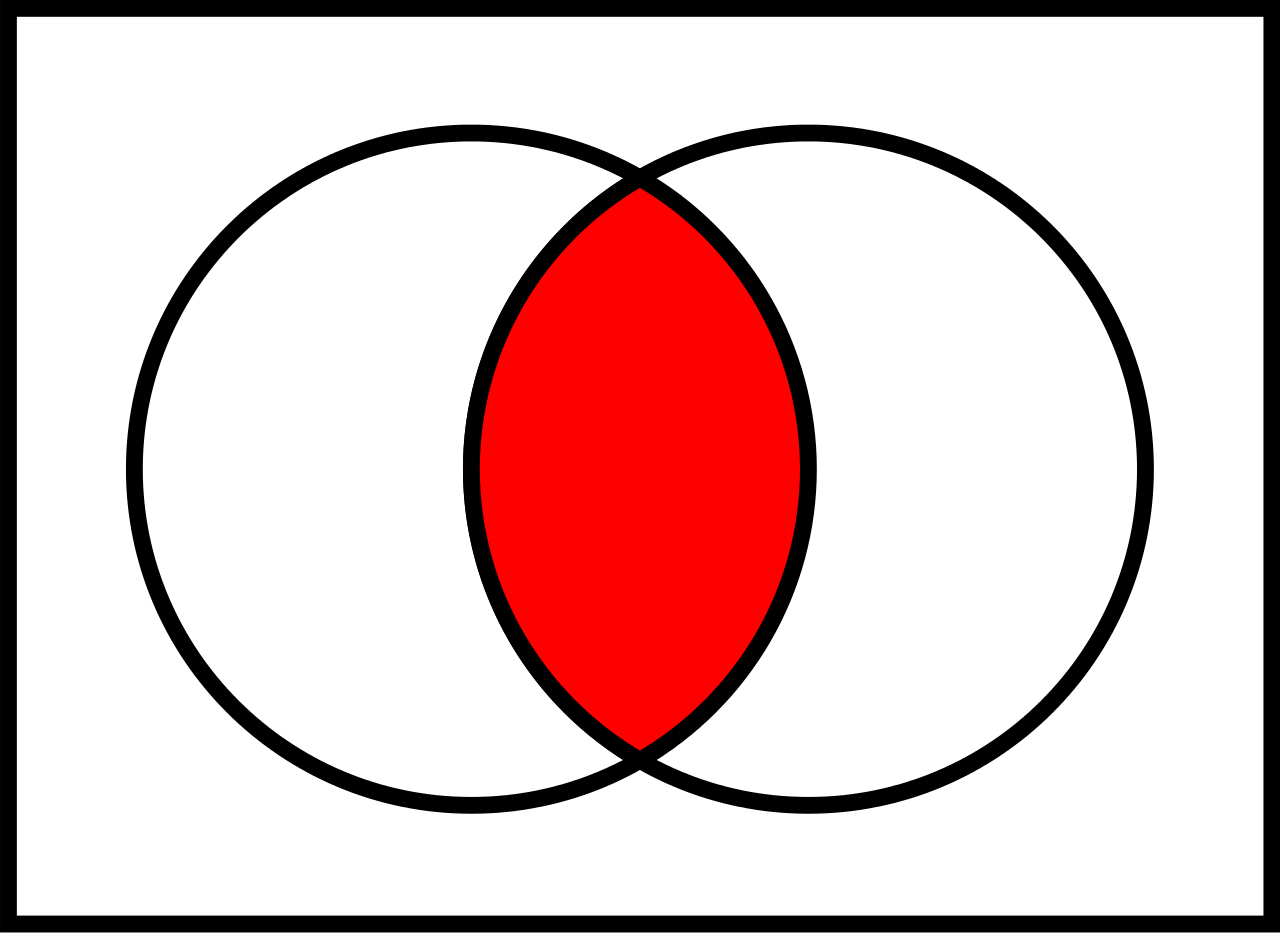
\includegraphics[scale=0.1]{images/intersect.png}
\caption{Диаграмма Венна для пересечения множеств}
\label{pic-intersect}
\end{figure}
\end{frame}

\begin{frame}{Бинарные операции}
\begin{block}{Объединение}
\[A\cap B := \{ x|x \in A \vee x \in B \}\].
\end{block}
\begin{figure}[h]
\centering
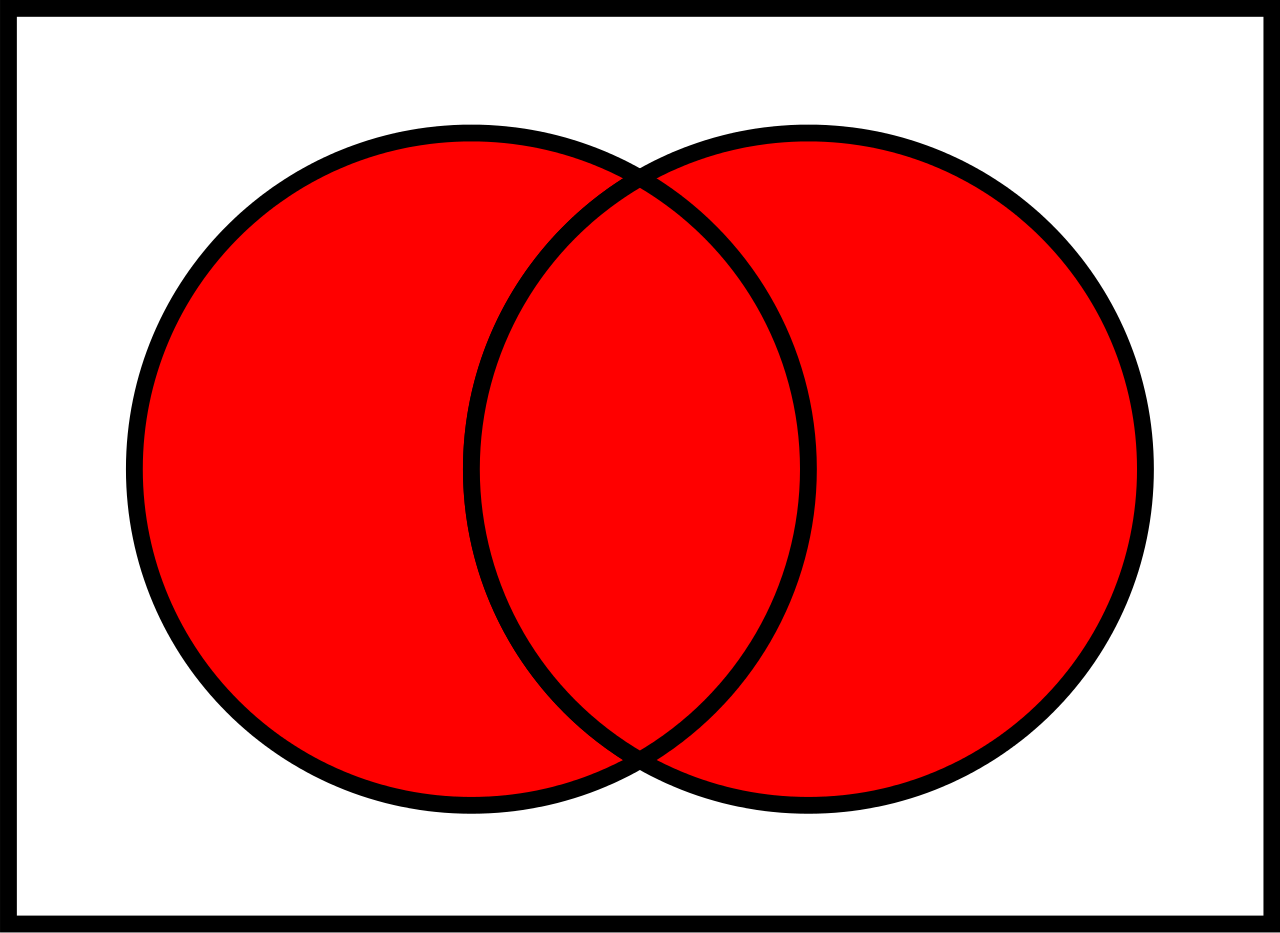
\includegraphics[scale=0.1]{images/union.png}
\caption{Диаграмма Венна для объединения множеств}
\label{pic-union}
\end{figure}
\end{frame}

\begin{frame}{Бинарные операции}
\begin{block}{Разность множеств}
\[A \setminus B := \{ x|x \in A \wedge x \notin B \}\].
\end{block}
\begin{figure}[h]
\centering
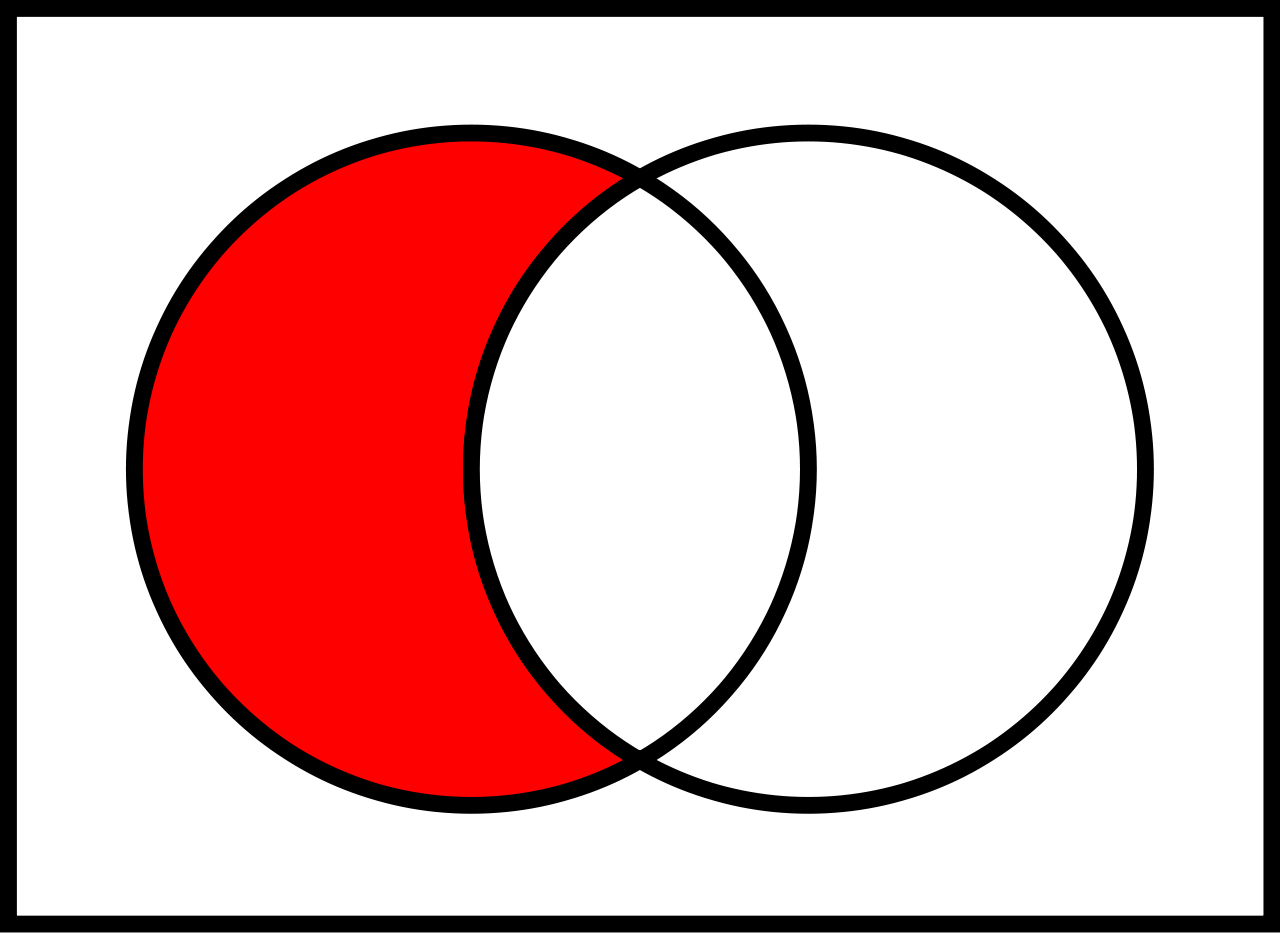
\includegraphics[scale=0.1]{images/sub.png}
\caption{Диаграмма Венна для разности множеств}
\label{pic-union}
\end{figure}
\end{frame}

\begin{frame}{Бинарные операции}
\begin{block}{Симметрическая разность множеств}
\[A \bigtriangleup B := (A \setminus B)\cup(B\setminus A)\].
\end{block}
\begin{figure}[h]
\centering
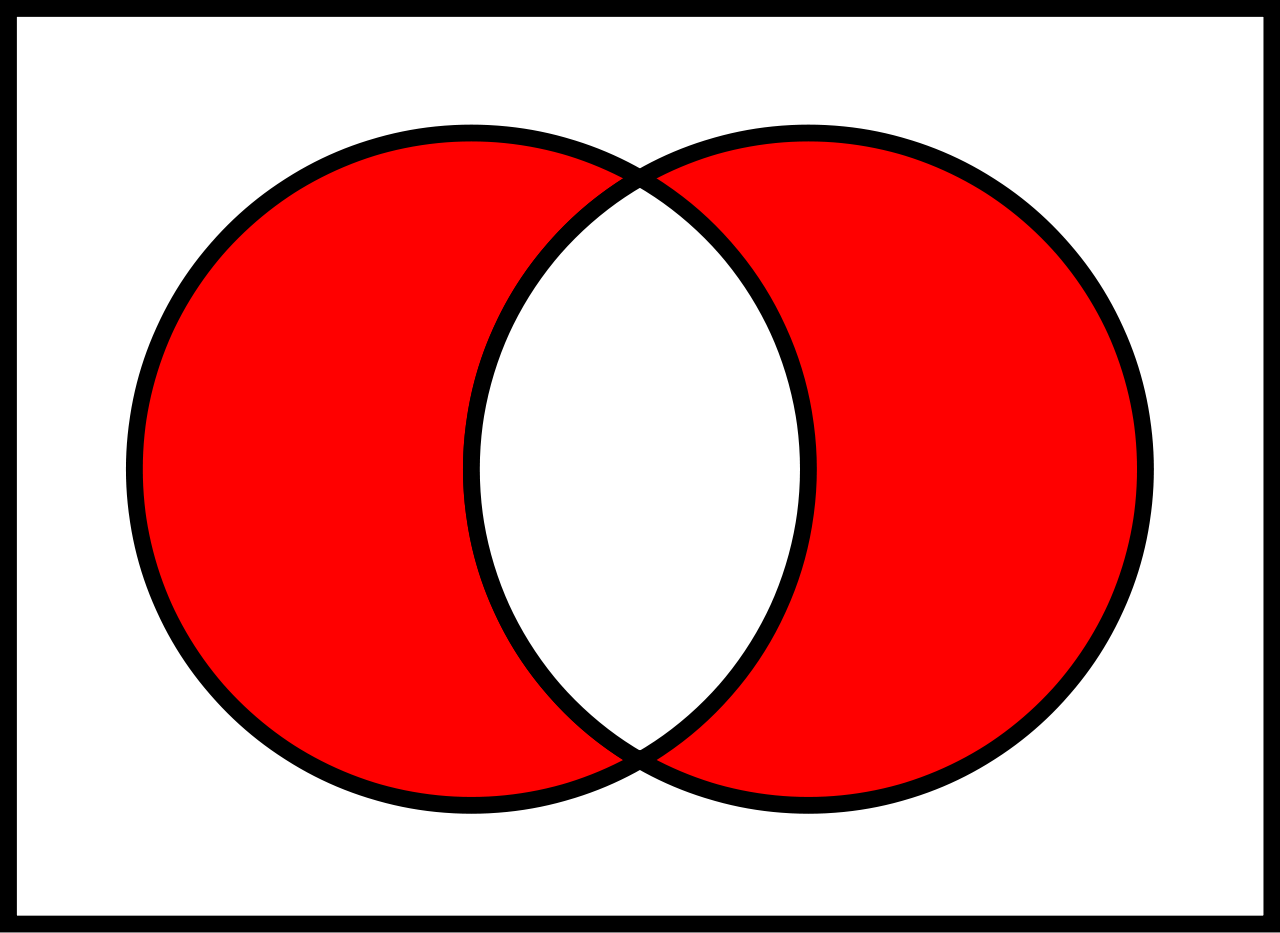
\includegraphics[scale=0.1]{images/xor.png}
\caption{Диаграмма Венна для симметрической разности множеств}
\label{pic-union}
\end{figure}
\end{frame}

\section{Множественный тип в языке Pascal}
\begin{frame}[fragile]
\begin{block}{Множество}
структура данных, представляющая ограниченную неупорядоченную совокупность различных элементов одного типа.
\end{block}
\begin{alltt}
1  a := []; //пустое множество
2  b := [2, 4, 7, 10]; //множество из четырех элементов целого типа
3  с := ['e', 'u', 'i', 'o', 'a', 'y']; //множество из шести символов
4  k := 15; d := [1, k, 2*k]; //множество трех элементов
5  e := [1..100];
6  f := [k..2*k];
7  g := ['A'..'Z', 'a'..'z'];
8  h := [1..1, 5..1]; //эквивалентно [1]
9  j := [5..1];//эквивалентно []
\end{alltt}
Порядок перечисления элементов в множестве не играет роли.
\begin{alltt}
10  m := [5, 3, 1]; //эквивалентно [1, 3, 5]
11  n := [1, z, 2*z]; //эквивалентно [1, 2] при z = 1
\end{alltt}
\end{frame}

\begin{frame}[fragile]
\begin{block}{Множественный тип (тип множества)}
структурный тип данных, значением которого является множество.
\end{block}
\begin{alltt}
  type ИмяТипа = set of БазовыйТип;
\end{alltt}
Базовый тип - любой порядковый (+ ограничения реализации Pascal).
\begin{alltt}
1  type 
2     TLetters = 'A'..'Z';
3     TLettersSet = set of TLetters;
4     TCharSet = set of char;  
5     TIndexSet = set of 1..100;
\end{alltt}
В программе могут быть заданы константы и переменные множественного типа.
\begin{alltt}
6  const 
7     Wowels = ['e', 'u', 'i', 'o', 'a', 'y'];
\end{alltt}
\end{frame}
   
\begin{frame}[fragile]
\begin{block}{Конструктор множества}
позволяет задать значение переменной или константы множественного типа.
\end{block}
\begin{alltt}
1  type TLetters = set of char;
2  var
3     EnglishCap, EnglishStr: TLetters;
4  begin
5     RussianCap := ['A'..'Z'];
6     EnglishStr := ['a'..'z'];
\end{alltt}
Переменные и типизированные константы могут участвовать в опрациях присваивания, если они 
принадлежат к идентичным типам.
\end{frame}  

\begin{frame}
\begin{block}{Операции над множествами}
\begin{itemize}
\item объединение [1, 2, 4] + [2, 4, 8]; //результат [1, 2, 4, 8];
\item пересечение [1, 2, 4] * [2, 4, 8]; //результат [2, 4];
\item разность [1, 2, 4] - [2, 4, 8]; //результат [1];
\end{itemize}
\end{block}
\begin{block}{Операции отношения}
\begin{itemize}
\item равенство (A = B);
\item неравенство (A <> B);
\item A содержится в B (A <= B);
\item A содержит B (A >= B);
\end{itemize}
\end{block}
\begin{block}{Принадлежность элемента множеству}
\begin{itemize}
\item x in A;
\end{itemize}
\end{block}
Приоритет операций: пересечение, (объединение, разность), сравнение и принадлежность
\end{frame}  

\begin{frame}[fragile]{Пример: вывести элементы множества}
\begin{alltt}
1  const
2    Low = 1;    //минимальное значение элемента множества
3    High = 32; //максимальное значение элемента множества
4  type 
5     TBase = Low..High; // базовый тип - отрезок Low..High    
6     TSet = set of TBase; //множественный тип
7  var
8     SimpleNumber: TSet; //множество чисел
9     Number: TBase; //переменная-элемент множества     
10 begin
11    SimpleNumber := [2, 3, 5, 7, 11, 13, 17, 23, 29, 31];
12    for Number := Low to High do
13      if Number in SimpleNumber then
14         write(Number:3);
\end{alltt}
\end{frame}   

\begin{frame}[fragile]{Пример: сформировать множество цифр числа}
\begin{alltt}
1  type TSet = set of 0..9; //множественный тип
2  var
3    DigitSet: TSet; //множество чисел
4    Digit: 0..9;   //переменная-элемент множества     
5    N, M: longint;  //иходное и вспомогательное число
6  begin
7    write('N = '); readln(N); M := N;
8    while M > 0 do begin
9      include(DigitSet, M mod 10);
10      M := M div 10;
11   end;  
12    for Digit := 0 to 9 do
13      if Digit in DigitSet then
14         write(Digit:2);
\end{alltt}
\end{frame}  

\begin{frame}[fragile]{Пример: ввести с клавиатуры множество символов}
\begin{alltt}
1 var
2   c: char;
3   s: set of char;
4
5 begin
6   write('Enter a string (Ctrl+Z - end if input): ');
7   s := [];
8   repeat
9     read(c);
10    if EOLN then
11      break;
12
13    include(s, c); //или так: s := s + [c];
14  until false;
15  readln;
\end{alltt}
\end{frame} 

\begin{frame}[fragile]{Пример: ввести из введенной последовательности только английские буквы}
\begin{alltt}
16  //пересечение множества s и множества английских букв
17  s := s * ['A'..'Z','a'..'z'];
18
19  //выводим множество
20  for c := chr(32) to chr(255) do
21    if c in s then
22      write(c, ' ');
23  writeln;
\end{alltt}
\end{frame}   

\begin{frame}[fragile]{Пример: вывести цифры, входящие в оба числа (M, N)}
\begin{alltt}
1 program set_02;
2 type
3  TBase = 0..9;
4
5 var
6  Digit: TBase;
7  SetM, SetN, ResultSet: set of TBase;
8  M, N, M1, N1: longint;
9
10 begin
11  write('Input M = ');
12  readln(M);
13  write('Input N = ');
14  readln(N);
15  writeln;
\end{alltt}
\end{frame}  

\begin{frame}[fragile]{Пример: вывести цифры, входящие в оба числа (M, N)}
\begin{alltt}
16  M1 := M; N1 := N;
17
18  SetM := [];
19  while M1 > 0 do
20  begin
21    SetM := SetM + [M1 mod 10];
22    M1 := M1 div 10;
23  end;
24
25  SetN := [];
26  while N1 > 0 do
27  begin
28    SetN := SetN + [N1 mod 10];
29    N1 := N1 div 10;
30  end;
31
32  ResultSet := SetM * SetN;
\end{alltt}
\end{frame}  

\begin{frame}[fragile]{Пример: вывести цифры, входящие в оба числа (M, N)}
\begin{alltt}
33  writeln('Digits in ', M, ':');
34  for Digit := 0 to 9 do
35    if Digit in SetM then
35      write(Digit, ' ');
37  
38  writeln; writeln('Digits in ', N, ':');
39  for Digit := 0 to 9 do
40    if Digit in SetN then
41      write(Digit, ' ');
42  
43  writeln; writeln('Digits in both numbers:');
44  for Digit := 0 to 9 do
45    if Digit in ResultSet then
46      write(Digit, ' ');
47  readln;
58 end.
\end{alltt}
\end{frame} 

\begin{frame}
\begin{block}{Упражнения}
\begin{itemize}
\item определить, является ли последовательность симоволов корректным идентификатором языка Pascal;
\item определить, из скольких различных цифр состоит число;
\item сформировать множество простых чисел, не превышающее N;
\item Вывести цифры, не входящие в десятичную запись числа.
\item Определить, можно ли из символов одного слова составить другое слово.
\item Определить повторяющиеся гласные буквы в тексте.
\item Определить, каких символов в тексте больше: гласных или согласных.
\item Вывести буквы, входящие в текст только один раз.
\item Вывести буквы, входящие в текст более одного раза.
\item Вывести буквы, входящие в текст ровно два раза.
\end{itemize}
\end{block}
\end{frame}    
  
\section*{Литература}
\begin{frame}   
\begin{enumerate}
\item Множество // Математическая энциклопедия (в 5 томах). — М.: Советская Энциклопедия, 1982. — Т. 3. — С. 762.
\item К. Куратовский, А. Мостовский. Теория множеств / Перевод с английского М. И. Кратко под редакцией А. Д. Тайманова. — М.: Мир, 1970. — 416 с.
\item Н. Бурбаки. Основания математики. Логика. Теория множеств // Очерки по истории математики / И. Г. Башмакова (перевод с французского). — М: Издательство иностранной литературы, 1963. — С. 37—53. — 292 с. — (Элементы математики).
\item Г. Кантор. Труды по теории множеств. — М.: Наука, 1985. — 430 с. — (Классики науки). — 3450 экз..
\end{enumerate}
\end{frame}   

\end{document}
